% Options for packages loaded elsewhere
\PassOptionsToPackage{unicode}{hyperref}
\PassOptionsToPackage{hyphens}{url}
\PassOptionsToPackage{dvipsnames,svgnames,x11names}{xcolor}
%
\documentclass[
  11pt,
]{article}
\usepackage{amsmath,amssymb}
\usepackage{lmodern}
\usepackage{iftex}
\ifPDFTeX
  \usepackage[T1]{fontenc}
  \usepackage[utf8]{inputenc}
  \usepackage{textcomp} % provide euro and other symbols
\else % if luatex or xetex
  \usepackage{unicode-math}
  \defaultfontfeatures{Scale=MatchLowercase}
  \defaultfontfeatures[\rmfamily]{Ligatures=TeX,Scale=1}
\fi
% Use upquote if available, for straight quotes in verbatim environments
\IfFileExists{upquote.sty}{\usepackage{upquote}}{}
\IfFileExists{microtype.sty}{% use microtype if available
  \usepackage[]{microtype}
  \UseMicrotypeSet[protrusion]{basicmath} % disable protrusion for tt fonts
}{}
\makeatletter
\@ifundefined{KOMAClassName}{% if non-KOMA class
  \IfFileExists{parskip.sty}{%
    \usepackage{parskip}
  }{% else
    \setlength{\parindent}{0pt}
    \setlength{\parskip}{6pt plus 2pt minus 1pt}}
}{% if KOMA class
  \KOMAoptions{parskip=half}}
\makeatother
\usepackage{xcolor}
\IfFileExists{xurl.sty}{\usepackage{xurl}}{} % add URL line breaks if available
\IfFileExists{bookmark.sty}{\usepackage{bookmark}}{\usepackage{hyperref}}
\hypersetup{
  pdftitle={Study of the effectiveness of selected data imputation techniques on the mobile phone parameters dataset},
  pdfauthor={Dawid Chomicz},
  colorlinks=true,
  linkcolor={blue},
  filecolor={Maroon},
  citecolor={Blue},
  urlcolor={Blue},
  pdfcreator={LaTeX via pandoc}}
\urlstyle{same} % disable monospaced font for URLs
\usepackage[margin=1in]{geometry}
\usepackage{longtable,booktabs,array}
\usepackage{calc} % for calculating minipage widths
% Correct order of tables after \paragraph or \subparagraph
\usepackage{etoolbox}
\makeatletter
\patchcmd\longtable{\par}{\if@noskipsec\mbox{}\fi\par}{}{}
\makeatother
% Allow footnotes in longtable head/foot
\IfFileExists{footnotehyper.sty}{\usepackage{footnotehyper}}{\usepackage{footnote}}
\makesavenoteenv{longtable}
\usepackage{graphicx}
\makeatletter
\def\maxwidth{\ifdim\Gin@nat@width>\linewidth\linewidth\else\Gin@nat@width\fi}
\def\maxheight{\ifdim\Gin@nat@height>\textheight\textheight\else\Gin@nat@height\fi}
\makeatother
% Scale images if necessary, so that they will not overflow the page
% margins by default, and it is still possible to overwrite the defaults
% using explicit options in \includegraphics[width, height, ...]{}
\setkeys{Gin}{width=\maxwidth,height=\maxheight,keepaspectratio}
% Set default figure placement to htbp
\makeatletter
\def\fps@figure{htbp}
\makeatother
\setlength{\emergencystretch}{3em} % prevent overfull lines
\providecommand{\tightlist}{%
  \setlength{\itemsep}{0pt}\setlength{\parskip}{0pt}}
\setcounter{secnumdepth}{-\maxdimen} % remove section numbering
\usepackage{setspace}
\usepackage{caption}
\captionsetup[figure]{labelformat=empty}
\usepackage{floatrow}
\floatsetup[figure]{capposition=top}
\usepackage{booktabs}
\usepackage{longtable}
\usepackage{array}
\usepackage{multirow}
\usepackage{wrapfig}
\usepackage{float}
\usepackage{colortbl}
\usepackage{pdflscape}
\usepackage{tabu}
\usepackage{threeparttable}
\usepackage{threeparttablex}
\usepackage[normalem]{ulem}
\usepackage{makecell}
\usepackage{xcolor}
\ifLuaTeX
  \usepackage{selnolig}  % disable illegal ligatures
\fi
\usepackage[]{biblatex}

\title{Study of the effectiveness of selected data imputation techniques on the mobile phone parameters dataset}
\author{Dawid Chomicz}
\date{2022-06-29}

\begin{document}
\maketitle

The aim of the study is to compare the effectiveness of selected data imputation techniques. For this purpose, the \emph{phone.csv} data set describing the technical parameters of mobile phones was used. The process of generating data deficiencies and imputating these deficiencies was simulated, and then the average descriptive statistics for each imputation technique used were estimated. The calculations were made with the R programming language.

\hypertarget{characteristics-of-the-dataset}{%
\subsection{Characteristics of the dataset}\label{characteristics-of-the-dataset}}

The data comes from the resources of the \href{https://www.kaggle.com/datasets/iabhishekofficial/mobile-price-classification?resource=download\&select=train.csv}{kaggle.com} site. The set contains 1000 observations in the form of numerical variables. Detailed description of each variable:

\begin{itemize}
\tightlist
\item
  \emph{battery} --- total battery capacity in mAh,
\item
  \emph{speed} -- processor speed,
\item
  \emph{fc} -- front camera megapixels,
\item
  \emph{memory} -- internal memory in GB,
\item
  \emph{weight} -- phone weight,
\item
  \emph{pc} -- main camera megapixels,
\item
  \emph{ram} -- RAM in MB,
\item
  \emph{sc\_h} -- screen height in cm,
\item
  \emph{sc\_w} -- screen width in cm,
\item
  \emph{talk\_t} -- maximum usage time in hours without recharging the battery.
\end{itemize}

\hypertarget{details-of-the-simulation-process}{%
\subsection{Details of the simulation process}\label{details-of-the-simulation-process}}

The performed simulation aims to compare the effectiveness of selected data imputation techniques on the same set of observations. For this purpose, an algorithm consisting of three steps was prepared:

\begin{enumerate}
\def\labelenumi{\arabic{enumi}.}
\tightlist
\item
  Generating MCAR (\emph{missing completely at random}) type missing data in the set, covering 20\% of the data without taking into account the first two variables.
\item
  Application of the following imputation techniques to the generated set: mean, median, regression, K nearest neighbors, random forest.
\item
  Calculation of statistics describing the structure of the dataset after imputation for each technique.
\end{enumerate}

The above algorithm was iterated a thousand times and the results of these iterations were averaged.

Parameters adopted for individual techniques:

\begin{itemize}
\tightlist
\item
  Regression -- generalized linear model with automatic selection of the linking function and distribution of the modeled variable, where the dependent variables were all variables with missing values, and the explanatory variables were the first two variables,
\item
  K najbliższych sąsiadów -- parameter \emph{k = 5},
\item
  Las losowy -- the formula for modeled and explanatory variables is the same as in regression.
\end{itemize}

\hypertarget{missing-data-characteristics}{%
\subsection{Missing data characteristics}\label{missing-data-characteristics}}

\begin{figure}

{\centering 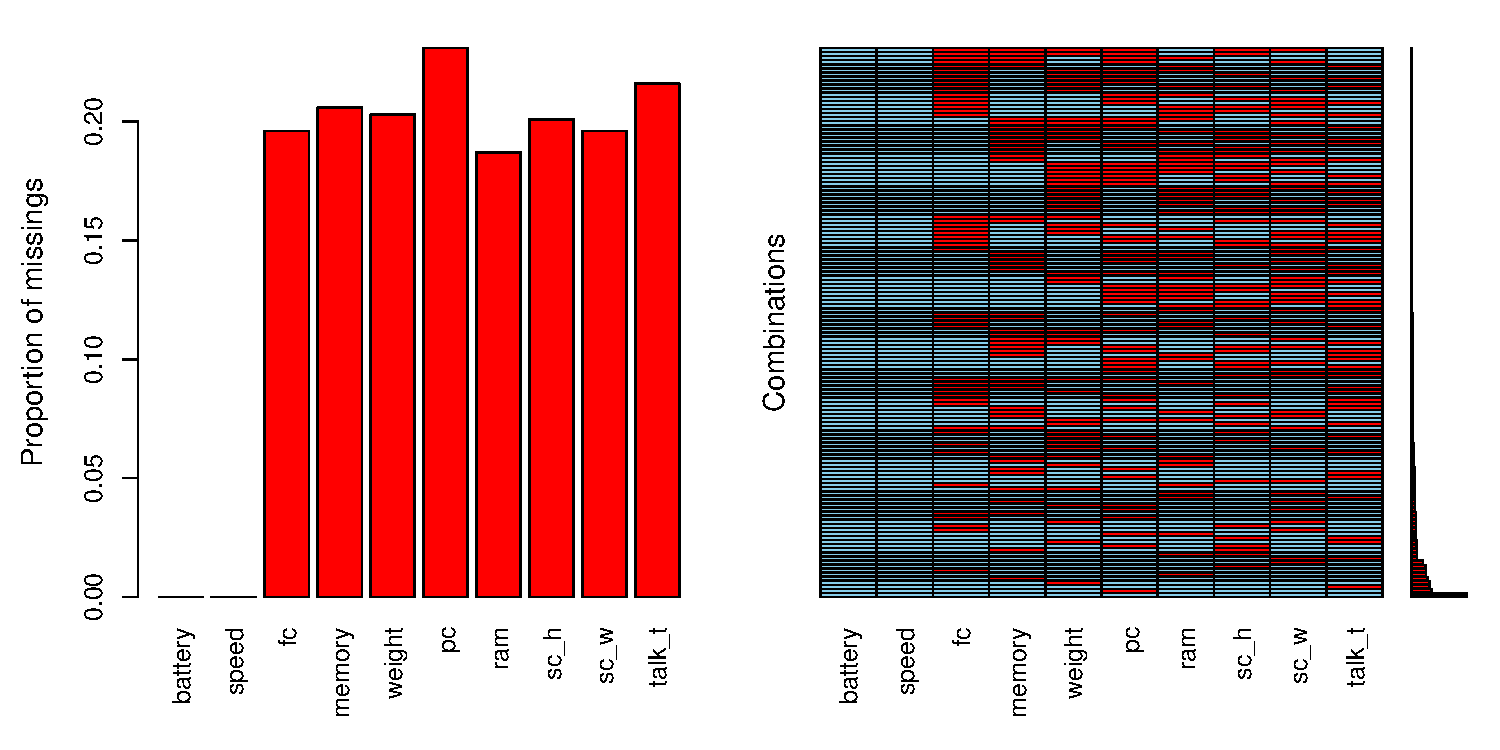
\includegraphics{report_files/figure-latex/unnamed-chunk-1-1} 

}

\caption{Figure 1. The frequency and distribution of missing data}\label{fig:unnamed-chunk-1}
\end{figure}

In the chart above, you can see the frequency and distribution of missing data in the generated dataset. The frequency as assumed fluctuates around 20\%. There are no deficiencies in the first two variables. Combinations od missing data do not show strong relations, although there is a slightly greater number of deficiency combinations between \emph{fc} and \emph{memory} and between \emph{memory} and \emph{weight} than in other cases.

\hypertarget{simulation-results}{%
\subsection{Simulation results}\label{simulation-results}}

The first table below lists the descriptive statistics for the initial, unchanged dataset. The following tables show the subtraction of the averaged statistics for simulated imputation techniques from the base set statistics. The * abs\_sum * column contains the sum of the absolute difference values for each statistic.
\newpage
\textbf{For initial data}

\begin{longtable}{lcccccccccc}
\toprule
  & battery & speed & fc & memory & weight & pc & ram & sc\_h & sc\_w & talk\_t\\
\midrule
\endfirsthead
\multicolumn{11}{@{}l}{\textit{(continued)}}\\
\toprule
  & battery & speed & fc & memory & weight & pc & ram & sc\_h & sc\_w & talk\_t\\
\midrule
\endhead

\endfoot
\bottomrule
\endlastfoot
\cellcolor{gray!15}{x\_sr} & \cellcolor{gray!15}{1248.51} & \cellcolor{gray!15}{1.54} & \cellcolor{gray!15}{4.59} & \cellcolor{gray!15}{33.65} & \cellcolor{gray!15}{139.51} & \cellcolor{gray!15}{10.05} & \cellcolor{gray!15}{2139.00} & \cellcolor{gray!15}{11.99} & \cellcolor{gray!15}{5.32} & \cellcolor{gray!15}{11.09}\\
Me & 1246.50 & 1.50 & 3.00 & 34.50 & 139.00 & 10.00 & 2153.50 & 12.00 & 5.00 & 11.00\\
\cellcolor{gray!15}{s} & \cellcolor{gray!15}{432.46} & \cellcolor{gray!15}{0.83} & \cellcolor{gray!15}{4.46} & \cellcolor{gray!15}{18.13} & \cellcolor{gray!15}{34.85} & \cellcolor{gray!15}{6.10} & \cellcolor{gray!15}{1088.09} & \cellcolor{gray!15}{4.32} & \cellcolor{gray!15}{4.24} & \cellcolor{gray!15}{5.50}\\
Vs & 0.35 & 0.54 & 0.97 & 0.54 & 0.25 & 0.61 & 0.51 & 0.36 & 0.80 & 0.50\\
\cellcolor{gray!15}{s\_x\_sr} & \cellcolor{gray!15}{13.68} & \cellcolor{gray!15}{0.03} & \cellcolor{gray!15}{0.14} & \cellcolor{gray!15}{0.57} & \cellcolor{gray!15}{1.10} & \cellcolor{gray!15}{0.19} & \cellcolor{gray!15}{34.41} & \cellcolor{gray!15}{0.14} & \cellcolor{gray!15}{0.13} & \cellcolor{gray!15}{0.17}\\
g1 & 0.04 & 0.19 & 0.99 & -0.07 & 0.01 & 0.00 & -0.05 & -0.04 & 0.78 & 0.02\\*
\end{longtable}

\textbf{Mean imputation}

\begin{longtable}[l]{lccccccccc}
\toprule
  & fc & memory & weight & pc & ram & sc\_h & sc\_w & talk\_t & abs\_sum\\
\midrule
\endfirsthead
\multicolumn{10}{@{}l}{\textit{(continued)}}\\
\toprule
  & fc & memory & weight & pc & ram & sc\_h & sc\_w & talk\_t & abs\_sum\\
\midrule
\endhead

\endfoot
\bottomrule
\endlastfoot
\cellcolor{gray!15}{x\_sr} & \cellcolor{gray!15}{0.00} & \cellcolor{gray!15}{-0.01} & \cellcolor{gray!15}{0.02} & \cellcolor{gray!15}{0.00} & \cellcolor{gray!15}{0.18} & \cellcolor{gray!15}{0.00} & \cellcolor{gray!15}{0.01} & \cellcolor{gray!15}{0.00} & \cellcolor{gray!15}{0.22}\\
Me & -1.59 & 0.84 & -0.49 & -0.06 & 14.69 & 0.00 & -0.31 & -0.09 & 18.06\\
\cellcolor{gray!15}{s} & \cellcolor{gray!15}{0.47} & \cellcolor{gray!15}{1.93} & \cellcolor{gray!15}{3.69} & \cellcolor{gray!15}{0.64} & \cellcolor{gray!15}{114.91} & \cellcolor{gray!15}{0.46} & \cellcolor{gray!15}{0.45} & \cellcolor{gray!15}{0.58} & \cellcolor{gray!15}{123.13}\\
Vs & 0.10 & 0.06 & 0.03 & 0.06 & 0.05 & 0.04 & 0.08 & 0.05 & 0.48\\
\cellcolor{gray!15}{s\_x\_sr} & \cellcolor{gray!15}{0.01} & \cellcolor{gray!15}{0.06} & \cellcolor{gray!15}{0.12} & \cellcolor{gray!15}{0.02} & \cellcolor{gray!15}{3.63} & \cellcolor{gray!15}{0.01} & \cellcolor{gray!15}{0.01} & \cellcolor{gray!15}{0.02} & \cellcolor{gray!15}{3.89}\\
g1 & -0.12 & 0.01 & 0.00 & 0.00 & 0.01 & 0.00 & -0.09 & 0.00 & 0.23\\*
\end{longtable}

\textbf{Median imputation}

\begin{longtable}[l]{lccccccccc}
\toprule
  & fc & memory & weight & pc & ram & sc\_h & sc\_w & talk\_t & abs\_sum\\
\midrule
\endfirsthead
\multicolumn{10}{@{}l}{\textit{(continued)}}\\
\toprule
  & fc & memory & weight & pc & ram & sc\_h & sc\_w & talk\_t & abs\_sum\\
\midrule
\endhead

\endfoot
\bottomrule
\endlastfoot
\cellcolor{gray!15}{x\_sr} & \cellcolor{gray!15}{0.23} & \cellcolor{gray!15}{-0.16} & \cellcolor{gray!15}{0.11} & \cellcolor{gray!15}{0.01} & \cellcolor{gray!15}{-2.41} & \cellcolor{gray!15}{0.00} & \cellcolor{gray!15}{0.14} & \cellcolor{gray!15}{0.02} & \cellcolor{gray!15}{3.09}\\
Me & -0.43 & 0.05 & -0.06 & 0.01 & 1.70 & 0.00 & 0.38 & 0.01 & 2.65\\
\cellcolor{gray!15}{s} & \cellcolor{gray!15}{0.44} & \cellcolor{gray!15}{1.92} & \cellcolor{gray!15}{3.68} & \cellcolor{gray!15}{0.64} & \cellcolor{gray!15}{114.87} & \cellcolor{gray!15}{0.46} & \cellcolor{gray!15}{0.44} & \cellcolor{gray!15}{0.58} & \cellcolor{gray!15}{123.03}\\
Vs & 0.05 & 0.06 & 0.03 & 0.06 & 0.05 & 0.04 & 0.06 & 0.05 & 0.40\\
\cellcolor{gray!15}{s\_x\_sr} & \cellcolor{gray!15}{0.01} & \cellcolor{gray!15}{0.06} & \cellcolor{gray!15}{0.12} & \cellcolor{gray!15}{0.02} & \cellcolor{gray!15}{3.63} & \cellcolor{gray!15}{0.01} & \cellcolor{gray!15}{0.01} & \cellcolor{gray!15}{0.02} & \cellcolor{gray!15}{3.89}\\
g1 & -0.26 & 0.04 & -0.01 & -0.01 & 0.01 & 0.01 & -0.19 & -0.01 & 0.53\\*
\end{longtable}

\textbf{Regression imputation}

\begin{longtable}[l]{lccccccccc}
\toprule
  & fc & memory & weight & pc & ram & sc\_h & sc\_w & talk\_t & abs\_sum\\
\midrule
\endfirsthead
\multicolumn{10}{@{}l}{\textit{(continued)}}\\
\toprule
  & fc & memory & weight & pc & ram & sc\_h & sc\_w & talk\_t & abs\_sum\\
\midrule
\endhead

\endfoot
\bottomrule
\endlastfoot
\cellcolor{gray!15}{x\_sr} & \cellcolor{gray!15}{0.00} & \cellcolor{gray!15}{-0.01} & \cellcolor{gray!15}{0.02} & \cellcolor{gray!15}{0.00} & \cellcolor{gray!15}{0.18} & \cellcolor{gray!15}{0.00} & \cellcolor{gray!15}{0.01} & \cellcolor{gray!15}{0.00} & \cellcolor{gray!15}{0.22}\\
Me & -1.48 & 0.75 & -0.44 & -0.02 & 12.44 & -0.01 & -0.12 & -0.03 & 15.28\\
\cellcolor{gray!15}{s} & \cellcolor{gray!15}{0.47} & \cellcolor{gray!15}{1.92} & \cellcolor{gray!15}{3.67} & \cellcolor{gray!15}{0.64} & \cellcolor{gray!15}{114.73} & \cellcolor{gray!15}{0.45} & \cellcolor{gray!15}{0.45} & \cellcolor{gray!15}{0.57} & \cellcolor{gray!15}{122.92}\\
Vs & 0.10 & 0.06 & 0.03 & 0.06 & 0.05 & 0.04 & 0.08 & 0.05 & 0.48\\
\cellcolor{gray!15}{s\_x\_sr} & \cellcolor{gray!15}{0.01} & \cellcolor{gray!15}{0.06} & \cellcolor{gray!15}{0.12} & \cellcolor{gray!15}{0.02} & \cellcolor{gray!15}{3.63} & \cellcolor{gray!15}{0.01} & \cellcolor{gray!15}{0.01} & \cellcolor{gray!15}{0.02} & \cellcolor{gray!15}{3.89}\\
g1 & -0.12 & 0.01 & 0.00 & 0.00 & 0.01 & 0.00 & -0.09 & 0.00 & 0.23\\*
\end{longtable}
\newpage

\textbf{K nearest neighbors imputation}

\begin{longtable}[l]{lccccccccc}
\toprule
  & fc & memory & weight & pc & ram & sc\_h & sc\_w & talk\_t & abs\_sum\\
\midrule
\endfirsthead
\multicolumn{10}{@{}l}{\textit{(continued)}}\\
\toprule
  & fc & memory & weight & pc & ram & sc\_h & sc\_w & talk\_t & abs\_sum\\
\midrule
\endhead

\endfoot
\bottomrule
\endlastfoot
\cellcolor{gray!15}{x\_sr} & \cellcolor{gray!15}{0.11} & \cellcolor{gray!15}{-0.02} & \cellcolor{gray!15}{-0.11} & \cellcolor{gray!15}{0.10} & \cellcolor{gray!15}{-3.20} & \cellcolor{gray!15}{0.04} & \cellcolor{gray!15}{0.05} & \cellcolor{gray!15}{-0.01} & \cellcolor{gray!15}{3.65}\\
Me & -0.67 & 0.14 & -0.32 & 0.08 & -2.97 & 0.00 & 0.27 & 0.02 & 4.47\\
\cellcolor{gray!15}{s} & \cellcolor{gray!15}{0.27} & \cellcolor{gray!15}{1.12} & \cellcolor{gray!15}{2.04} & \cellcolor{gray!15}{0.32} & \cellcolor{gray!15}{61.13} & \cellcolor{gray!15}{0.22} & \cellcolor{gray!15}{0.24} & \cellcolor{gray!15}{0.31} & \cellcolor{gray!15}{65.66}\\
Vs & 0.04 & 0.03 & 0.01 & 0.03 & 0.03 & 0.02 & 0.04 & 0.03 & 0.22\\
\cellcolor{gray!15}{s\_x\_sr} & \cellcolor{gray!15}{0.01} & \cellcolor{gray!15}{0.04} & \cellcolor{gray!15}{0.06} & \cellcolor{gray!15}{0.01} & \cellcolor{gray!15}{1.93} & \cellcolor{gray!15}{0.01} & \cellcolor{gray!15}{0.01} & \cellcolor{gray!15}{0.01} & \cellcolor{gray!15}{2.08}\\
g1 & -0.05 & 0.01 & 0.00 & -0.03 & 0.01 & -0.01 & -0.03 & 0.00 & 0.15\\*
\end{longtable}

\textbf{Random forest imputation}

\begin{longtable}[l]{lccccccccc}
\toprule
  & fc & memory & weight & pc & ram & sc\_h & sc\_w & talk\_t & abs\_sum\\
\midrule
\endfirsthead
\multicolumn{10}{@{}l}{\textit{(continued)}}\\
\toprule
  & fc & memory & weight & pc & ram & sc\_h & sc\_w & talk\_t & abs\_sum\\
\midrule
\endhead

\endfoot
\bottomrule
\endlastfoot
\cellcolor{gray!15}{x\_sr} & \cellcolor{gray!15}{-0.01} & \cellcolor{gray!15}{-0.01} & \cellcolor{gray!15}{-0.01} & \cellcolor{gray!15}{0.00} & \cellcolor{gray!15}{0.57} & \cellcolor{gray!15}{0.00} & \cellcolor{gray!15}{0.00} & \cellcolor{gray!15}{0.00} & \cellcolor{gray!15}{0.59}\\
Me & -1.00 & 0.32 & -0.58 & 0.02 & 4.94 & 0.00 & 0.01 & -0.01 & 6.89\\
\cellcolor{gray!15}{s} & \cellcolor{gray!15}{0.42} & \cellcolor{gray!15}{1.72} & \cellcolor{gray!15}{3.30} & \cellcolor{gray!15}{0.58} & \cellcolor{gray!15}{102.12} & \cellcolor{gray!15}{0.40} & \cellcolor{gray!15}{0.40} & \cellcolor{gray!15}{0.51} & \cellcolor{gray!15}{109.45}\\
Vs & 0.09 & 0.05 & 0.02 & 0.06 & 0.05 & 0.03 & 0.07 & 0.05 & 0.43\\
\cellcolor{gray!15}{s\_x\_sr} & \cellcolor{gray!15}{0.01} & \cellcolor{gray!15}{0.05} & \cellcolor{gray!15}{0.10} & \cellcolor{gray!15}{0.02} & \cellcolor{gray!15}{3.23} & \cellcolor{gray!15}{0.01} & \cellcolor{gray!15}{0.01} & \cellcolor{gray!15}{0.02} & \cellcolor{gray!15}{3.46}\\
g1 & -0.08 & 0.01 & 0.00 & 0.00 & 0.00 & 0.00 & -0.06 & 0.00 & 0.15\\*
\end{longtable}

The table below compares all the sums of the absolute values of the estimated differences for each simulated imputation technique.

\begin{longtable}[l]{lccccc}
\toprule
  & mean & median & regression & kNN & random forest\\
\midrule
\endfirsthead
\multicolumn{6}{@{}l}{\textit{(continued)}}\\
\toprule
  & mean & median & regression & kNN & random forest\\
\midrule
\endhead

\endfoot
\bottomrule
\endlastfoot
\cellcolor{gray!15}{x\_sr} & \cellcolor{gray!15}{0.22} & \cellcolor{gray!15}{3.09} & \cellcolor{gray!15}{0.22} & \cellcolor{gray!15}{3.65} & \cellcolor{gray!15}{0.59}\\
Me & 18.06 & 2.65 & 15.28 & 4.47 & 6.89\\
\cellcolor{gray!15}{s} & \cellcolor{gray!15}{123.13} & \cellcolor{gray!15}{123.03} & \cellcolor{gray!15}{122.92} & \cellcolor{gray!15}{65.66} & \cellcolor{gray!15}{109.45}\\
Vs & 0.48 & 0.40 & 0.48 & 0.22 & 0.43\\
\cellcolor{gray!15}{s\_x\_sr} & \cellcolor{gray!15}{3.89} & \cellcolor{gray!15}{3.89} & \cellcolor{gray!15}{3.89} & \cellcolor{gray!15}{2.08} & \cellcolor{gray!15}{3.46}\\
g1 & 0.23 & 0.53 & 0.23 & 0.15 & 0.15\\*
\end{longtable}

Comparing the above tables, it can be concluded that:

In the case of the arithmetic mean for the studied variables, imputations with regression and random forest turned out to be the closest.

In the case of the median for the studied variables, the imputations with the median and the K nearest neighbors turned out to be the most similar.

In the case of the standard deviation for the studied variables, the imputations of K nearest neighbors and the random forest turned out to be the most similar.

In the case of the coefficient of variation for the studied variables, the imputations of K nearest neighbors and the random forest turned out to be the most similar.

In the case of the standard error of the mean for the studied variables, the imputations of K nearest neighbors and the random forest turned out to be the closest.

In the case of the asymmetry coefficient for the studied variables, the imputations of K nearest neighbors and random forest turned out to be the closest.

\textbf{Conclusion}: The imputation technique that produces results on average closest to the original set values is the K nearest neighbors. In the case of the mean and the median, better results were achieved by the mean and median imputations respectively, which seems natural due to the specificity of these measures.

\printbibliography

\end{document}
